\documentclass{article}
\usepackage{enumerate}
\usepackage{amsmath}
\usepackage{amssymb}
\usepackage{graphicx}
\usepackage{subfigure}
\usepackage{geometry}
\usepackage{caption}
\usepackage{indentfirst}
\usepackage{fancyhdr}
\usepackage{ulem}
\usepackage{multirow}
\usepackage{tabu}
\usepackage{array}
\usepackage{minted}

\date{}
\pagestyle{fancy}
\fancyhead{}
\fancyhead[C]{
\includegraphics[width=\linewidth]{ji_header.png}}
\fancyfoot[C]{\thepage}
\renewcommand{\headrulewidth}{0pt}
\addtolength{\headheight}{4\baselineskip}
\geometry{top=4cm,bottom=4.0cm}
\begin{document}

\vspace*{3mm}

\begin{minipage}{0.6\linewidth}
\ 
\end{minipage}
\hfill
\begin{minipage}{0.38\linewidth}
\begin{center}
\huge\bfseries
Lab Report \\[8mm]
\fontsize{100pt}{\baselineskip}\selectfont
4
\end{center}
\end{minipage}

\vspace*{1cm}

{\huge\bfseries
\uline{UM-SJTU Joint Institute \phantom{xxxxxxxxxxxx}}
\vspace*{2mm}

Ve270 Introduction to Logic Design
}	

\vspace*{2cm}
\begin{center}
\LARGE
by \\[2mm]
\begin{tabular}{ll}
Liu Yihao & 515370910207 \\
Ma ShiYao & 515370910157
\end{tabular}

\vspace*{2cm}
Date: 2017-06-20
\end{center}

\vspace*{2cm}
\begin{center}
\Huge\bfseries
Design of a Simple Counter
\end{center}

\newpage

\section{Objectives}
To design a  FSM-Counter by both schematics and  HDL modeling.

\section{Problem Definition}
To design a  4-bit up/down synchronous binary counter which is capable for 0 to 15 using 4 flip-flops sharing the same clock signal. It should be able to count up and down, controlled by an 1-bit inputting called “up/down” implemented by a switch. It is to increment when “up/down” signal is a binary 1 and to decrement if the signal is 0. There should be another input called “Reset” provided by a button. The counter should be 0 if the signal “Reset” is 1.

\section{System Partitioning}
\begin{enumerate}
\item Switches and buttons. Used to input signals like “Up/down mode choose”, “Reset” and the signals to count.
\item Inside circuit. It is designed by using ISE and used to process the input signals and come up with output signals.
\item LED. The output the digits got by the circuit by illuminating different segments of LED. The rule of illumination according to the output digits is the same as Lab 2.
\end{enumerate}

\section{Design Entry}
The function of this system was shown in Table \ref{function-table}.

\begin{table}[!hbtp]
\centering
\begin{tabular}{|p{2cm}<{\centering}|p{2cm}<{\centering}|p{4cm}<{\centering}|}
\hline
\multicolumn{2}{|c|}{Input signals} & \multirow{2}{*}{Output (Count)}  \\\cline{1-2}
Reset & Up/down & \\\hline
1 & X & 0 \\\hline
0 & 0 & Count+1 \\\hline
0 & 1 & Count-1 \\\hline
\end{tabular}
\caption{Function table}
\label{function-table}
\end{table}

According to the Table \ref{function-table}, we designed the ALU circuit, shown in Figure \ref{design-counter}. \\

\begin{figure}[!htbp]
\centering
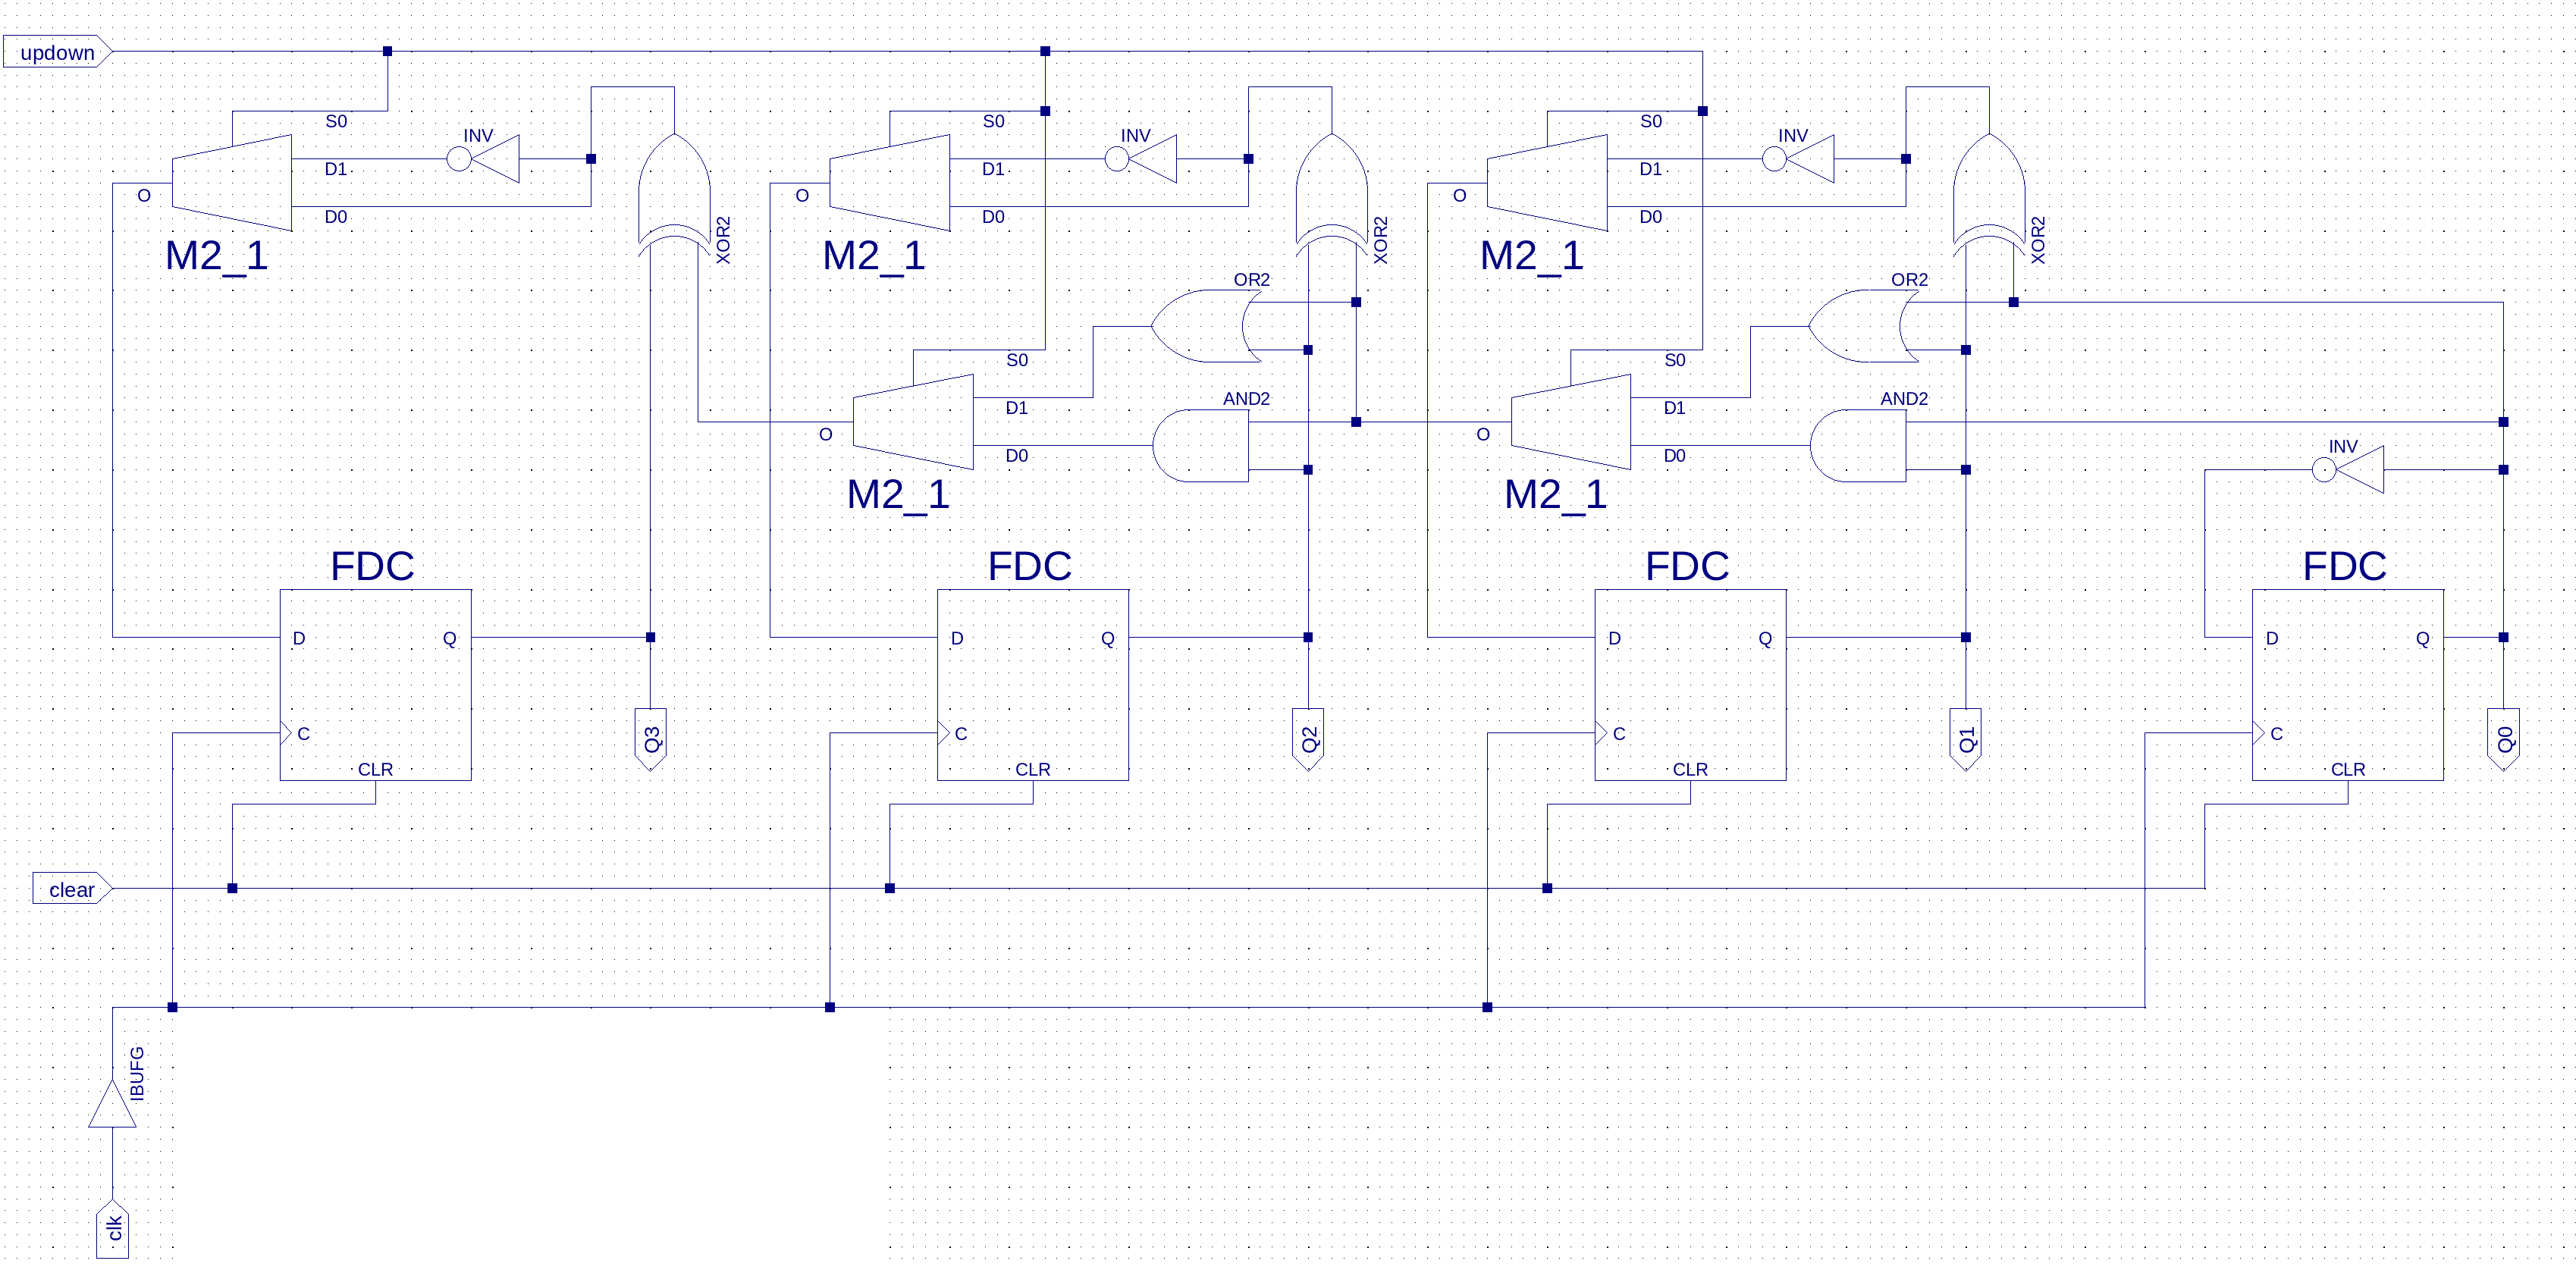
\includegraphics[width=0.95\linewidth]{counter.png}
\caption{Schematics design of Counter}
\label{design-counter}
\end{figure}

\newpage
The rule of illumination according to the output (from Lab 2 SSD Driver) was shown in Figure \ref{ssd-fig} and Table \ref{ssd-table}.

\begin{figure}[!htbp]
\centering
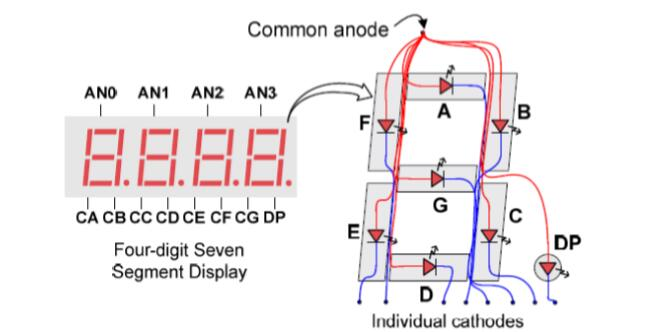
\includegraphics[width=0.65\linewidth]{SSD.jpg}
\caption{SSD Definition}
\label{ssd-fig}
\end{figure}

\begin{table}[!hbtp]
\centering
\begin{tabular}{|p{1cm}<{\centering}|p{1cm}<{\centering}|p{1cm}<{\centering}|p{1cm}<{\centering}|p{1cm}<{\centering}|p{1cm}<{\centering}|p{1cm}<{\centering}|p{1cm}<{\centering}|}
\hline
\multirow{2}{*}{Input} & \multicolumn{7}{c|}{ Outputs(LED segments) }\\\cline{2-8}
& CA & CB & CC & CD & CE & CF & CG \\\hline
0000 & 0 & 0 & 0 & 0 & 0 & 0 & 1 \\\hline
0001 & 1 & 0 & 0 & 1 & 1 & 1 & 1 \\\hline
0010 & 0 & 0 & 1 & 0 & 0 & 1 & 0 \\\hline
0011 & 0 & 0 & 0 & 0 & 1 & 1 & 0 \\\hline
0100 & 1 & 0 & 0 & 1 & 1 & 0 & 0 \\\hline
0101 & 0 & 1 & 0 & 0 & 1 & 0 & 0 \\\hline
0110 & 0 & 1 & 0 & 0 & 0 & 0 & 0 \\\hline
0111 & 0 & 0 & 0 & 1 & 1 & 1 & 1 \\\hline
1000 & 0 & 0 & 0 & 0 & 0 & 0 & 0 \\\hline
1010 & 0 & 0 & 0 & 0 & 1 & 0 & 0 \\\hline
1011 & 1 & 1 & 0 & 0 & 0 & 0 & 0 \\\hline
1100 & 0 & 1 & 1 & 0 & 0 & 0 & 1 \\\hline
1101 & 1 & 0 & 0 & 0 & 0 & 1 & 0 \\\hline
1110 & 0 & 1 & 1 & 0 & 0 & 0 & 0 \\\hline
1111 & 0 & 1 & 1 & 1 & 0 & 0 & 0 \\\hline
\end{tabular}
\caption{SSD truth table}
\label{ssd-table}
\end{table}



\newpage

\section{Test Plan}
\begin{center}
\begin{tabular}{|m{3cm}<{\centering}|m{10cm}|}
\hline
Test content & \multicolumn{1}{c|}{Test method} \\\hline
 & \multirow{6}{10cm}{Switch the counter on up/down mode, then input an “count” signal, observe the output digit. \\[1em] 
If the output digit gets larger by 1 in “up” mode/smaller by 1 in “down” mode, it passes the test, otherwise it fails.} \\
Up Counter & \\ & \\\cline{1-1} & \\
Down Counter & \\ & \\\hline
Reset button & Input an “reset” signal by the  button, then observe the output digit.
If the output digit becomes 0, it passes the test, otherwise it fails. \\\hline
\end{tabular}
\end{center}

\section{Simulation Results}
We simulated the result of the overall system with input values in Table \ref{function-table}, shown in Figure \ref{simulation}.

\begin{figure}[!htbp]
\centering
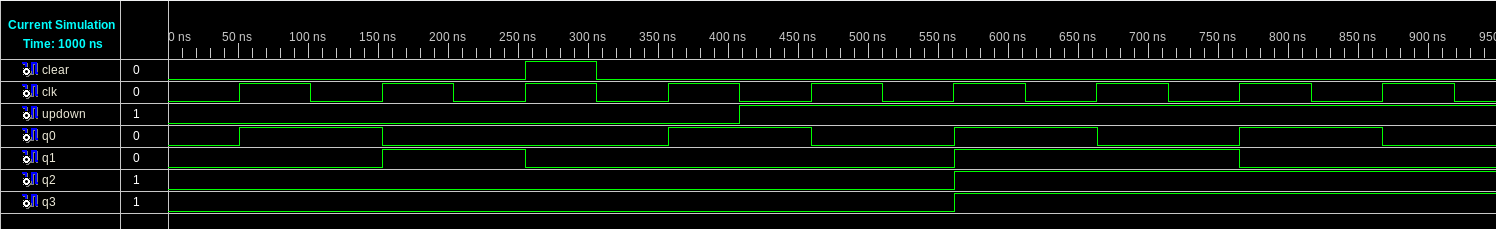
\includegraphics[width=0.9\linewidth]{simulation.png}
\caption{Simulation of Counter}
\label{simulation}
\end{figure}

We found the values in the simulation identical to Table \ref{def-table}.



\section{Conclusion}
In this lab, we successfully finished it finally, but we also met with some problems in the process. Some existing modules in ISE will cause error in the simulation and pace process, such as the inverse-4 and mux-4, so we have to build a new module ourselves. We practiced build a ALU with 2-bit select input signal and four kinds of  algorithms.

\section{Appendix}
The schematics of our design had been submitted to canvas before.

The verilog file is shown here:
\inputminted{verilog}{../lab4/counter_verilog.v}

The verilog testbench file is shown here:
\inputminted{verilog}{../lab4/counter_test.v}


\end{document}